\scanpage{98}

\uline{Dém} \quad On est ramené au cas où
$Y$ est \inserted{noeth} \unsure{strictemt|strictement} local, et par transitivité au cas
où $X$ est de dim relative 1 sur $Y$.\thinspace\ldots\thinspace.

\figure{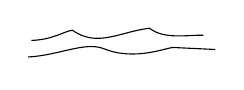
\begin{tikzpicture}[x=.5cm,y=.5cm]
\draw (0,0)..controls(.55,.02)and(.8,.22)..(1.04,.26)..controls(1.68,-.19)and(2.24,.22)..(3,.31)..controls(3.38,.01)and(4,.15)..(4.37,.13);
\draw (-.08,-.42)..controls(.7,-.38)and(1.36,-.02)..(1.84,-.21)..controls(2.65,-.54)and(3.47,-.16)..(3.62,-.18)--(4.67,-.23);
\end{tikzpicture}}

\uline{Applications} 1) Soit $f:X\longrightarrow Y$ un morphisme qu. cpt
\llap{\smash{\rule[-2.1ex]{.4pt}{4.6ex}}\hspace{.65em}}qu. sép. Alors les $R^i\unsure{f|f_*}(F)$ \unsure{commutent|hom. naturel|homomorphisme|localement constant} \unsure{à|:}
\unsure{tt|toute|par} extension lisse de la base.

\deleted{2) Soit $X$}

2) $X$ préschéma sur un corps sép. clos. Alors
pour $k'/k$ ext. sép. clos, et tt $F$ de
torsion sur $X$ premier \deleted{\unsure{à}} à car. de $k$, on
a

\[ H^i(X,F)\xrightarrow{\sim}H^i(X',F') \]

(Étendre au $H^1$ et $H^2$ non commutatifs \ldots)\unsure{.|,}

3) Si $X$ lisse sur $S$, $Y$ sous-schéma lisse,
calcul des $\underline H^i_Y(F)$, $F$ loc constant sur
$X$ premier aux car. résiduelles (\uline{th. de
pureté relatif}).

% archive sheet number: 97
